\chapter{Chapter XLIII}

\begin{verse}
Be Mowbray's sins so heavy in his bosom,\\
That they may break his foaming courser's back,\\
And throw the rider headlong in the lists,\\
A caitiff recreant!\\!
\attrib{--Richard II}
\end{verse}

\lettrine{O}{ur} scene now returns to the exterior of the Castle,
or Preceptory, of
Templestowe, about the hour when the bloody die was to be cast for the
life or death of Rebecca. It was a scene of bustle and life, as if the
whole vicinity had poured forth its inhabitants to a village wake, or
rural feast. But the earnest desire to look on blood and death, is not
peculiar to those dark ages; though in the gladiatorial exercise of
single combat and general tourney, they were habituated to the bloody
spectacle of brave men falling by each other's hands. Even in our own
days, when morals are better understood, an execution, a bruising match,
a riot, or a meeting of radical reformers, collects, at considerable
hazard to themselves, immense crowds of spectators, otherwise little
interested, except to see how matters are to be conducted, or whether
the heroes of the day are, in the heroic language of insurgent tailors,
flints or dunghills.

The eyes, therefore, of a very considerable multitude, were bent on the
gate of the Preceptory of Templestowe, with the purpose of witnessing
the procession; while still greater numbers had already surrounded the
tiltyard belonging to that establishment. This enclosure was formed on a
piece of level ground adjoining to the Preceptory, which had been
levelled with care, for the exercise of military and chivalrous sports.
It occupied the brow of a soft and gentle eminence, was carefully
palisaded around, and, as the Templars willingly invited spectators to
be witnesses of their skill in feats of chivalry, was amply supplied
with galleries and benches for their use.

On the present occasion, a throne was erected for the Grand Master at
the east end, surrounded with seats of distinction for the Preceptors
and Knights of the Order. Over these floated the sacred standard, called
``Le Beau-seant'', which was the ensign, as its name was the battle-cry,
of the Templars.

At the opposite end of the lists was a pile of faggots, so arranged
around a stake, deeply fixed in the ground, as to leave a space for the
victim whom they were destined to consume, to enter within the fatal
circle, in order to be chained to the stake by the fetters which hung
ready for that purpose. Beside this deadly apparatus stood four black
slaves, whose colour and African features, then so little known in
England, appalled the multitude, who gazed on them as on demons employed
about their own diabolical exercises. These men stirred not, excepting
now and then, under the direction of one who seemed their chief, to
shift and replace the ready fuel. They looked not on the multitude. In
fact, they seemed insensible of their presence, and of every thing save
the discharge of their own horrible duty.

And when, in speech with each other, they expanded their blubber lips,
and showed their white fangs, as if they grinned at the thoughts of the
expected tragedy, the startled commons could scarcely help believing
that they were actually the familiar spirits with whom the witch had
communed, and who, her time being out, stood ready to assist in her
dreadful punishment. They whispered to each other, and communicated all
the feats which Satan had performed during that busy and unhappy period,
not failing, of course, to give the devil rather more than his due.

``Have you not heard, Father Dennet,'' quoth one boor to another
advanced in years, ``that the devil has carried away bodily the great
Saxon Thane, Athelstane of Coningsburgh?''

``Ay, but he brought him back though, by the blessing of God and Saint
Dunstan.''

``How's that?'' said a brisk young fellow, dressed in a green cassock
embroidered with gold, and having at his heels a stout lad bearing a
harp upon his back, which betrayed his vocation. The Minstrel seemed of
no vulgar rank; for, besides the splendour of his gaily braidered
doublet, he wore around his neck a silver chain, by which hung the
``wrest'', or key, with which he tuned his harp. On his right arm was a
silver plate, which, instead of bearing, as usual, the cognizance or
badge of the baron to whose family he belonged, had barely the word
SHERWOOD engraved upon it.--``How mean you by that?'' said the gay
Minstrel, mingling in the conversation of the peasants; ``I came to seek
one subject for my rhyme, and, by'r Lady, I were glad to find two.''

``It is well avouched,'' said the elder peasant, ``that after Athelstane
of Coningsburgh had been dead four weeks--''

``That is impossible,'' said the Minstrel; ``I saw him in life at the
Passage of Arms at Ashby-de-la-Zouche.''

``Dead, however, he was, or else translated,'' said the younger peasant;
``for I heard the Monks of Saint Edmund's singing the death's hymn for
him; and, moreover, there was a rich death-meal and dole at the Castle
of Coningsburgh, as right was; and thither had I gone, but for Mabel
Parkins, who--''

``Ay, dead was Athelstane,'' said the old man, shaking his head, ``and
the more pity it was, for the old Saxon blood--''

``But, your story, my masters--your story,'' said the Minstrel, somewhat
impatiently.

``Ay, ay--construe us the story,'' said a burly Friar, who stood beside
them, leaning on a pole that exhibited an appearance between a pilgrim's
staff and a quarter-staff, and probably acted as either when occasion
served,--``Your story,'' said the stalwart churchman; ``burn not
daylight about it--we have short time to spare.''

``An please your reverence,'' said Dennet, ``a drunken priest came to
visit the Sacristan at Saint Edmund's---''

``It does not please my reverence,'' answered the churchman, ``that
there should be such an animal as a drunken priest, or, if there were,
that a layman should so speak him. Be mannerly, my friend, and conclude
the holy man only wrapt in meditation, which makes the head dizzy and
foot unsteady, as if the stomach were filled with new wine--I have felt
it myself.''

``Well, then,'' answered Father Dennet, ``a holy brother came to visit
the Sacristan at Saint Edmund's--a sort of hedge-priest is the visitor,
and kills half the deer that are stolen in the forest, who loves the
tinkling of a pint-pot better than the sacring-bell, and deems a flitch
of bacon worth ten of his breviary; for the rest, a good fellow and a
merry, who will flourish a quarter-staff, draw a bow, and dance a
Cheshire round, with e'er a man in Yorkshire.''

``That last part of thy speech, Dennet,'' said the Minstrel, ``has saved
thee a rib or twain.''

``Tush, man, I fear him not,'' said Dennet; ``I am somewhat old and
stiff, but when I fought for the bell and ram at Doncaster--''

``But the story--the story, my friend,'' again said the Minstrel.

``Why, the tale is but this--Athelstane of Coningsburgh was buried at
Saint Edmund's.''

``That's a lie, and a loud one,'' said the Friar, ``for I saw him borne
to his own Castle of Coningsburgh.''

``Nay, then, e'en tell the story yourself, my masters,'' said Dennet,
turning sulky at these repeated contradictions; and it was with some
difficulty that the boor could be prevailed on, by the request of his
comrade and the Minstrel, to renew his tale.--``These two `sober'
friars,'' said he at length, ``since this reverend man will needs have
them such, had continued drinking good ale, and wine, and what not, for
the best part for a summer's day, when they were aroused by a deep
groan, and a clanking of chains, and the figure of the deceased
Athelstane entered the apartment, saying, `Ye evil shep-herds!--'\,''

``It is false,'' said the Friar, hastily, ``he never spoke a word.''

``So ho! Friar Tuck,'' said the Minstrel, drawing him apart from the
rustics; ``we have started a new hare, I find.''

``I tell thee, Allan-a-Dale,'' said the Hermit, ``I saw Athelstane of
Coningsburgh as much as bodily eyes ever saw a living man. He had his
shroud on, and all about him smelt of the sepulchre--A butt of sack will
not wash it out of my memory.''

``Pshaw!'' answered the Minstrel; ``thou dost but jest with me!''

``Never believe me,'' said the Friar, ``an I fetched not a knock at him
with my quarter-staff that would have felled an ox, and it glided
through his body as it might through a pillar of smoke!''

``By Saint Hubert,'' said the Minstrel, ``but it is a wondrous tale, and
fit to be put in metre to the ancient tune, `Sorrow came to the old
Friar.'\,''

``Laugh, if ye list,'' said Friar Tuck; ``but an ye catch me singing on
such a theme, may the next ghost or devil carry me off with him
headlong! No, no--I instantly formed the purpose of assisting at some
good work, such as the burning of a witch, a judicial combat, or the
like matter of godly service, and therefore am I here.''

As they thus conversed, the heavy bell of the church of Saint Michael of
Templestowe, a venerable building, situated in a hamlet at some distance
from the Preceptory, broke short their argument. One by one the sullen
sounds fell successively on the ear, leaving but sufficient space for
each to die away in distant echo, ere the air was again filled by
repetition of the iron knell. These sounds, the signal of the
approaching ceremony, chilled with awe the hearts of the assembled
multitude, whose eyes were now turned to the Preceptory, expecting the
approach of the Grand Master, the champion, and the criminal.

At length the drawbridge fell, the gates opened, and a knight, bearing
the great standard of the Order, sallied from the castle, preceded by
six trumpets, and followed by the Knights Preceptors, two and two, the
Grand Master coming last, mounted on a stately horse, whose furniture
was of the simplest kind. Behind him came Brian de Bois-Guilbert, armed
cap-a-pie in bright armour, but without his lance, shield, and sword,
which were borne by his two esquires behind him. His face, though partly
hidden by a long plume which floated down from his barrel-cap, bore a
strong and mingled expression of passion, in which pride seemed to
contend with irresolution. He looked ghastly pale, as if he had not
slept for several nights, yet reined his pawing war-horse with the
habitual ease and grace proper to the best lance of the Order of the
Temple. His general appearance was grand and commanding; but, looking at
him with attention, men read that in his dark features, from which they
willingly withdrew their eyes.

On either side rode Conrade of Mont-Fitchet, and Albert de Malvoisin,
who acted as godfathers to the champion. They were in their robes of
peace, the white dress of the Order. Behind them followed other
Companions of the Temple, with a long train of esquires and pages clad
in black, aspirants to the honour of being one day Knights of the Order.
After these neophytes came a guard of warders on foot, in the same sable
livery, amidst whose partisans might be seen the pale form of the
accused, moving with a slow but undismayed step towards the scene of her
fate. She was stript of all her ornaments, lest perchance there should
be among them some of those amulets which Satan was supposed to bestow
upon his victims, to deprive them of the power of confession even when
under the torture. A coarse white dress, of the simplest form, had been
substituted for her Oriental garments; yet there was such an exquisite
mixture of courage and resignation in her look, that even in this garb,
and with no other ornament than her long black tresses, each eye wept
that looked upon her, and the most hardened bigot regretted the fate
that had converted a creature so goodly into a vessel of wrath, and a
waged slave of the devil.

A crowd of inferior personages belonging to the Preceptory followed the
victim, all moving with the utmost order, with arms folded, and looks
bent upon the ground.

This slow procession moved up the gentle eminence, on the summit of
which was the tiltyard, and, entering the lists, marched once around
them from right to left, and when they had completed the circle, made a
halt. There was then a momentary bustle, while the Grand Master and all
his attendants, excepting the champion and his godfathers, dismounted
from their horses, which were immediately removed out of the lists by
the esquires, who were in attendance for that purpose.

The unfortunate Rebecca was conducted to the black chair placed near the
pile. On her first glance at the terrible spot where preparations were
making for a death alike dismaying to the mind and painful to the body,
she was observed to shudder and shut her eyes, praying internally
doubtless, for her lips moved though no speech was heard. In the space
of a minute she opened her eyes, looked fixedly on the pile as if to
familiarize her mind with the object, and then slowly and naturally
turned away her head.

Meanwhile, the Grand Master had assumed his seat; and when the chivalry
of his order was placed around and behind him, each in his due rank, a
loud and long flourish of the trumpets announced that the Court were
seated for judgment. Malvoisin, then, acting as godfather of the
champion, stepped forward, and laid the glove of the Jewess, which was
the pledge of battle, at the feet of the Grand Master.

``Valorous Lord, and reverend Father,'' said he, ``here standeth the
good Knight, Brian de Bois-Guilbert, Knight Preceptor of the Order of
the Temple, who, by accepting the pledge of battle which I now lay at
your reverence's feet, hath become bound to do his devoir in combat this
day, to maintain that this Jewish maiden, by name Rebecca, hath justly
deserved the doom passed upon her in a Chapter of this most Holy Order
of the Temple of Zion, condemning her to die as a sorceress;--here, I
say, he standeth, such battle to do, knightly and honourable, if such be
your noble and sanctified pleasure.''

``Hath he made oath,'' said the Grand Master, ``that his quarrel is just
and honourable? Bring forward the Crucifix and the `Te igitur'.''

``Sir, and most reverend father,'' answered Malvoisin, readily, ``our
brother here present hath already sworn to the truth of his accusation
in the hand of the good Knight Conrade de Mont-Fitchet; and otherwise he
ought not to be sworn, seeing that his adversary is an unbeliever, and
may take no oath.''

This explanation was satisfactory, to Albert's great joy; for the wily
knight had foreseen the great difficulty, or rather impossibility, of
prevailing upon Brian de Bois-Guilbert to take such an oath before the
assembly, and had invented this excuse to escape the necessity of his
doing so.

The Grand Master, having allowed the apology of Albert Malvoisin,
commanded the herald to stand forth and do his devoir. The trumpets then
again flourished, and a herald, stepping forward, proclaimed
aloud,--``Oyez, oyez, oyez.--Here standeth the good Knight, Sir Brian de
Bois-Guilbert, ready to do battle with any knight of free blood, who
will sustain the quarrel allowed and allotted to the Jewess Rebecca, to
try by champion, in respect of lawful essoine of her own body; and to
such champion the reverend and valorous Grand Master here present allows
a fair field, and equal partition of sun and wind, and whatever else
appertains to a fair combat.'' The trumpets again sounded, and there was
a dead pause of many minutes.

``No champion appears for the appellant,'' said the Grand Master. ``Go,
herald, and ask her whether she expects any one to do battle for her in
this her cause.'' The herald went to the chair in which Rebecca was
seated, and Bois-Guilbert suddenly turning his horse's head toward that
end of the lists, in spite of hints on either side from Malvoisin and
Mont-Fitchet, was by the side of Rebecca's chair as soon as the herald.

``Is this regular, and according to the law of combat?'' said Malvoisin,
looking to the Grand Master.

``Albert de Malvoisin, it is,'' answered Beaumanoir; ``for in this
appeal to the judgment of God, we may not prohibit parties from having
that communication with each other, which may best tend to bring forth
the truth of the quarrel.''

In the meantime, the herald spoke to Rebecca in these terms:--``Damsel,
the Honourable and Reverend the Grand Master demands of thee, if thou
art prepared with a champion to do battle this day in thy behalf, or if
thou dost yield thee as one justly condemned to a deserved doom?''

``Say to the Grand Master,'' replied Rebecca, ``that I maintain my
innocence, and do not yield me as justly condemned, lest I become guilty
of mine own blood. Say to him, that I challenge such delay as his forms
will permit, to see if God, whose opportunity is in man's extremity,
will raise me up a deliverer; and when such uttermost space is passed,
may His holy will be done!'' The herald retired to carry this answer to
the Grand Master.

``God forbid,'' said Lucas Beaumanoir, ``that Jew or Pagan should
impeach us of injustice!--Until the shadows be cast from the west to the
eastward, will we wait to see if a champion shall appear for this
unfortunate woman. When the day is so far passed, let her prepare for
death.''

The herald communicated the words of the Grand Master to Rebecca, who
bowed her head submissively, folded her arms, and, looking up towards
heaven, seemed to expect that aid from above which she could scarce
promise herself from man. During this awful pause, the voice of
Bois-Guilbert broke upon her ear--it was but a whisper, yet it startled
her more than the summons of the herald had appeared to do.

``Rebecca,'' said the Templar, ``dost thou hear me?''

``I have no portion in thee, cruel, hard-hearted man,'' said the
unfortunate maiden.

``Ay, but dost thou understand my words?'' said the Templar; ``for the
sound of my voice is frightful in mine own ears. I scarce know on what
ground we stand, or for what purpose they have brought us hither.--This
listed space--that chair--these faggots--I know their purpose, and yet
it appears to me like something unreal--the fearful picture of a vision,
which appals my sense with hideous fantasies, but convinces not my
reason.''

``My mind and senses keep touch and time,'' answered Rebecca, ``and tell
me alike that these faggots are destined to consume my earthly body, and
open a painful but a brief passage to a better world.''

``Dreams, Rebecca,--dreams,'' answered the Templar; ``idle visions,
rejected by the wisdom of your own wiser Sadducees. Hear me, Rebecca,''
he said, proceeding with animation; ``a better chance hast thou for life
and liberty than yonder knaves and dotard dream of. Mount thee behind me
on my steed--on Zamor, the gallant horse that never failed his rider. I
won him in single fight from the Soldan of Trebizond--mount, I say,
behind me--in one short hour is pursuit and enquiry far behind--a new
world of pleasure opens to thee--to me a new career of fame. Let them
speak the doom which I despise, and erase the name of Bois-Guilbert from
their list of monastic slaves! I will wash out with blood whatever blot
they may dare to cast on my scutcheon.''

\begin{figure}
    \centering
    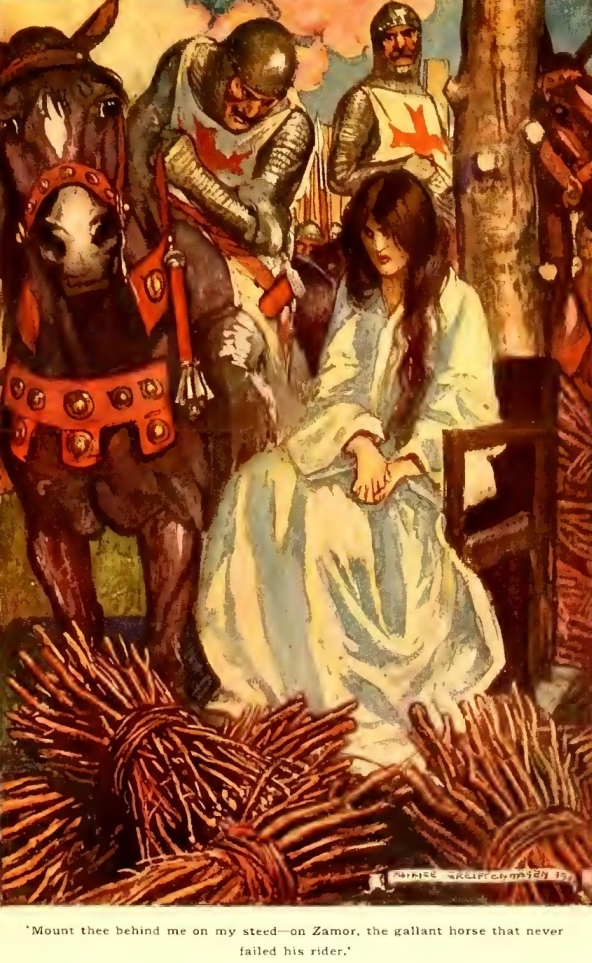
\includegraphics[height=.9\textheight]{ivanhoe/0581m}
    \caption{`Mount thee behind me on my steed--on Zamor, the gallant
    horse that never failed his rider.'}
\end{figure}

``Tempter,'' said Rebecca, ``begone!--Not in this last extremity canst
thou move me one hair's-breadth from my resting place--surrounded as I
am by foes, I hold thee as my worst and most deadly enemy--avoid thee,
in the name of God!''

Albert Malvoisin, alarmed and impatient at the duration of their
conference, now advanced to interrupt it.

``Hath the maiden acknowledged her guilt?'' he demanded of
Bois-Guilbert; ``or is she resolute in her denial?''

``She is indeed resolute,'' said Bois-Guilbert.

``Then,'' said Malvoisin, ``must thou, noble brother, resume thy place
to attend the issue--The shades are changing on the circle of the
dial--Come, brave Bois-Guilbert--come, thou hope of our holy Order, and
soon to be its head.''

As he spoke in this soothing tone, he laid his hand on the knight's
bridle, as if to lead him back to his station.

``False villain! what meanest thou by thy hand on my rein?'' said Sir
Brian, angrily. And shaking off his companion's grasp, he rode back to
the upper end of the lists.

``There is yet spirit in him,'' said Malvoisin apart to Mont-Fitchet,
``were it well directed--but, like the Greek fire, it burns whatever
approaches it.''

The Judges had now been two hours in the lists, awaiting in vain the
appearance of a champion.

``And reason good,'' said Friar Tuck, ``seeing she is a Jewess--and yet,
by mine Order, it is hard that so young and beautiful a creature should
perish without one blow being struck in her behalf! Were she ten times a
witch, provided she were but the least bit of a Christian, my
quarter-staff should ring noon on the steel cap of yonder fierce
Templar, ere he carried the matter off thus.''

It was, however, the general belief that no one could or would appear
for a Jewess, accused of sorcery; and the knights, instigated by
Malvoisin, whispered to each other, that it was time to declare the
pledge of Rebecca forfeited. At this instant a knight, urging his horse
to speed, appeared on the plain advancing towards the lists. A hundred
voices exclaimed, ``A champion! a champion!'' And despite the
prepossessions and prejudices of the multitude, they shouted unanimously
as the knight rode into the tiltyard. The second glance, however, served
to destroy the hope that his timely arrival had excited. His horse,
urged for many miles to its utmost speed, appeared to reel from fatigue,
and the rider, however undauntedly he presented himself in the lists,
either from weakness, weariness, or both, seemed scarce able to support
himself in the saddle.

To the summons of the herald, who demanded his rank, his name, and
purpose, the stranger knight answered readily and boldly, ``I am a good
knight and noble, come hither to sustain with lance and sword the just
and lawful quarrel of this damsel, Rebecca, daughter of Isaac of York;
to uphold the doom pronounced against her to be false and truthless, and
to defy Sir Brian de Bois-Guilbert, as a traitor, murderer, and liar; as
I will prove in this field with my body against his, by the aid of God,
of Our Lady, and of Monseigneur Saint George, the good knight.''

``The stranger must first show,'' said Malvoisin, ``that he is good
knight, and of honourable lineage. The Temple sendeth not forth her
champions against nameless men.''

``My name,'' said the Knight, raising his helmet, ``is better known, my
lineage more pure, Malvoisin, than thine own. I am Wilfred of Ivanhoe.''

``I will not fight with thee at present,'' said the Templar, in a
changed and hollow voice. ``Get thy wounds healed, purvey thee a better
horse, and it may be I will hold it worth my while to scourge out of
thee this boyish spirit of bravado.''

``Ha! proud Templar,'' said Ivanhoe, ``hast thou forgotten that twice
didst thou fall before this lance? Remember the lists at Acre--remember
the Passage of Arms at Ashby--remember thy proud vaunt in the halls of
Rotherwood, and the gage of your gold chain against my reliquary, that
thou wouldst do battle with Wilfred of Ivanhoe, and recover the honour
thou hadst lost! By that reliquary and the holy relic it contains, I
will proclaim thee, Templar, a coward in every court in Europe--in every
Preceptory of thine Order--unless thou do battle without farther
delay.''

Bois-Guilbert turned his countenance irresolutely towards Rebecca, and
then exclaimed, looking fiercely at Ivanhoe, ``Dog of a Saxon! take thy
lance, and prepare for the death thou hast drawn upon thee!''

``Does the Grand Master allow me the combat?'' said Ivanhoe.

``I may not deny what thou hast challenged,'' said the Grand Master,
``provided the maiden accepts thee as her champion. Yet I would thou
wert in better plight to do battle. An enemy of our Order hast thou ever
been, yet would I have thee honourably met with.''

``Thus--thus as I am, and not otherwise,'' said Ivanhoe; ``it is the
judgment of God--to his keeping I commend myself.--Rebecca,'' said he,
riding up to the fatal chair, ``dost thou accept of me for thy
champion?''

``I do,'' she said--``I do,'' fluttered by an emotion which the fear of
death had been unable to produce, ``I do accept thee as the champion
whom Heaven hath sent me. Yet, no--no--thy wounds are uncured--Meet not
that proud man--why shouldst thou perish also?''

But Ivanhoe was already at his post, and had closed his visor, and
assumed his lance. Bois-Guilbert did the same; and his esquire remarked,
as he clasped his visor, that his face, which had, notwithstanding the
variety of emotions by which he had been agitated, continued during the
whole morning of an ashy paleness, was now become suddenly very much
flushed.

The herald, then, seeing each champion in his place, uplifted his voice,
repeating thrice--``Faites vos devoirs, preux chevaliers!'' After the
third cry, he withdrew to one side of the lists, and again proclaimed,
that none, on peril of instant death, should dare, by word, cry, or
action, to interfere with or disturb this fair field of combat. The
Grand Master, who held in his hand the gage of battle, Rebecca's glove,
now threw it into the lists, and pronounced the fatal signal words,
``Laissez aller''.

The trumpets sounded, and the knights charged each other in full career.
The wearied horse of Ivanhoe, and its no less exhausted rider, went
down, as all had expected, before the well-aimed lance and vigorous
steed of the Templar. This issue of the combat all had foreseen; but
although the spear of Ivanhoe did but, in comparison, touch the shield
of Bois-Guilbert, that champion, to the astonishment of all who beheld
it reeled in his saddle, lost his stirrups, and fell in the lists.

Ivanhoe, extricating himself from his fallen horse, was soon on foot,
hastening to mend his fortune with his sword; but his antagonist arose
not. Wilfred, placing his foot on his breast, and the sword's point to
his throat, commanded him to yield him, or die on the spot.
Bois-Guilbert returned no answer.

``Slay him not, Sir Knight,'' cried the Grand Master, ``unshriven and
unabsolved--kill not body and soul! We allow him vanquished.''

He descended into the lists, and commanded them to unhelm the conquered
champion. His eyes were closed--the dark red flush was still on his
brow. As they looked on him in astonishment, the eyes opened--but they
were fixed and glazed. The flush passed from his brow, and gave way to
the pallid hue of death. Unscathed by the lance of his enemy, he had
died a victim to the violence of his own contending passions.

``This is indeed the judgment of God,'' said the Grand Master, looking
upwards--``\,`Fiat voluntas tua!'\,''
